\documentclass{article}

% Language setting
% Replace `english' with e.g. `spanish' to change the document language
\usepackage[french]{babel}

% Set page size and margins
% Replace `letterpaper' with`a4paper' for UK/EU standard size
\usepackage[letterpaper,top=3cm,bottom=2cm,left=3cm,right=3cm,marginparwidth=1.75cm]{geometry}

% Useful packages
\usepackage{amsmath}
\usepackage{graphicx}
\usepackage[colorlinks=true, allcolors=blue]{hyperref}
\usepackage[T1]{fontenc}
\usepackage{ragged2e}
\usepackage{mathtools}
\usepackage{graphicx}
\usepackage{float}
\usepackage{subcaption}
\usepackage{listings}
\usepackage{xcolor}
\graphicspath{ {./images/} }



\begin{document}


\begin{figure}[t]
\centering\includegraphics[width=5cm]{inp_n7.png}
\end{figure}

\title{\vspace{4cm} \textbf{Projet Modélisation géométrique}
\\ Option longue 2 : Un autre modèle de surface de subdivision (Butterfly)}
\author{Alice Devilder \\ Nicolas Catoni}

\date{\vspace{7cm} Département Sciences du Numérique - Deuxième année \\
HPC et Big Data \\ 2022-2023 }

\maketitle

\begin{center}
 \rule{0.5\linewidth}{1pt}
 \end{center}

 

\newpage

\section{Introduction}

Pour ce projet, nous avons choisi d'implémenter un modèle de représentation de surfaces à patches triangulaires interpolantes, aussi appelé interpolation de Butterfly. 

\section{Explication du modèle}

La méthode interpolante de Butterfly consiste à transformer récursivement chaque face triangulaire du polyhèdre de contrôle en un patch de 4 triangles interpolant les anciens points de contrôle. La règle pour insérer les nouveaux points est une règle à huit points basées sur la configuration décrite dans la figure ci-dessus. Celle-ci ressemble à un papillon d'où le nom de la méthode. \\

\begin{figure}[h]
\centering
    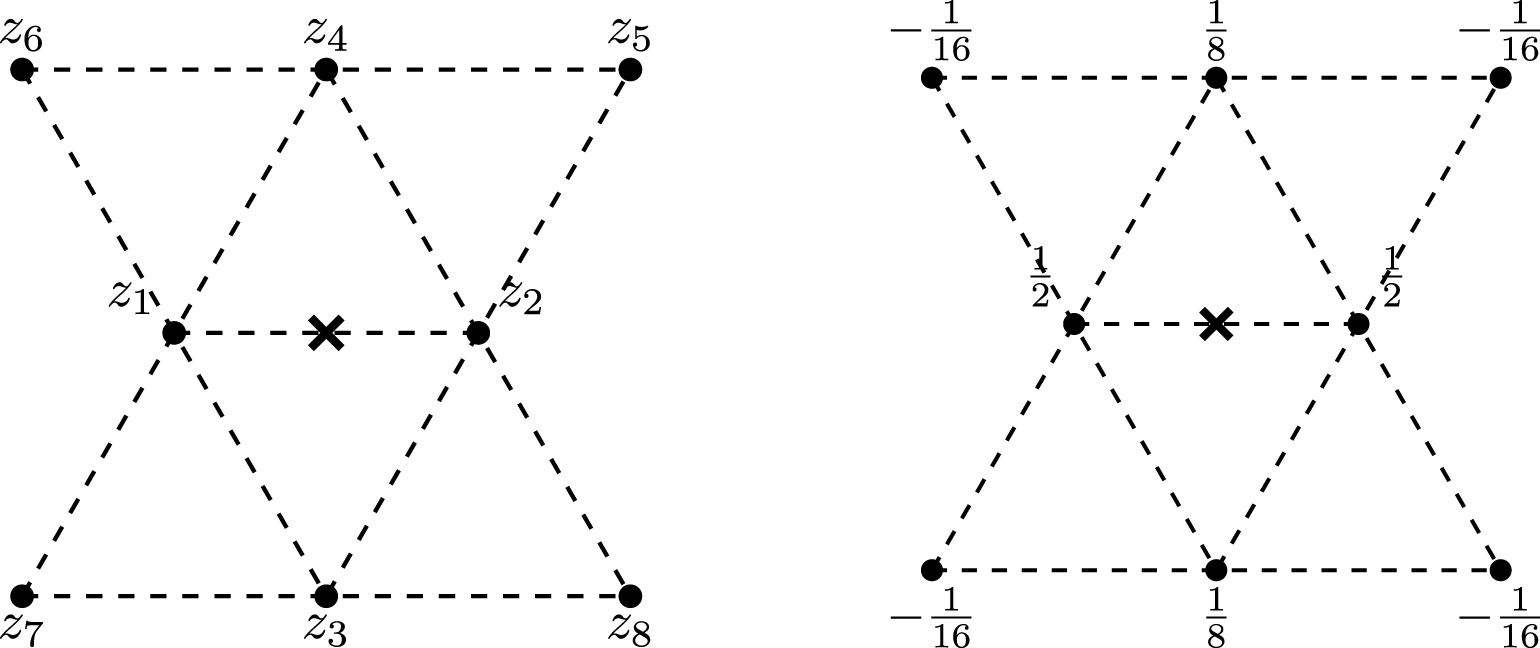
\includegraphics[width=10cm]{img_butterfly_2.jpg}
    \caption{Configuration des points pour le calcul du nouveau point pour une tension $\omega = \frac{1}{16}$}
\end{figure}


Pour obtenir la surface la plus lisse, il a été montré empiriquement que $\omega = \frac{1}{16}$. Plus généralement, le nouveau point $p^{k+1}$, qui correspond au milieu du segment $(z_1^k, z_2^k)$, est calculé de la façon suivante : \\
$$
\bar{p}^{k+1} = \frac{1}{2}(\bar{z_1}^{k}+\bar{z_2}^{k}) + 2 \omega (\bar{z_3}^{k} + \bar{z_4}^{k}) -\omega(\bar{z_5}^{k} + \bar{z_6}^{k} + \bar{z_7}^{k} + \bar{z_8}^{k})
$$\\
où $\bar{p}$ correspond à une des coordonnées du point $p$ et la valeur de tension $\omega$ vaut dans notre exemple $\frac{1}{16}$.

\section{Intérêts et avantages de ce modèle}

L'interpolation de Butterfly permet une interpolation rapide et efficace par calculs simple à chaque itération. De plus, elle nécessite une faible quantité de mémoire car elle ne stocke que les valeurs intermédiaires nécessaires aux calculs.\\

De plus, l'interpolation de Butterfly peut fournir une approximation précise de surfaces complexes à partir d'un ensemble limité de points de contrôle. Cela permet de représenter des surfaces lisses et détaillées, même avec un nombre réduit de données.

\section{Les limites de ce modèle}

Cependant, l'interpolation de Butterfly est plus adaptée aux surfaces régulières et lisses qu'aux surfaces présentant des caractéristiques topologiques complexes. Cette méthode peut rencontrer des difficultés lorsque la surface présente des singularités, des bords ou des formes non régulières. A ce moment là, on pourrait utiliser des algorithmes de Butterfly modifié mais d'autres algorithmes seraient plus efficaces. \\

Par ailleurs, comme toute méthode d'interpolation, le schéma de Butterfly dépend fortement de la disposition des points de contrôle. Une mauvaise répartition des points de contrôle peut entraîner une mauvaise approximation de la surface et des artefacts visuels indésirables. \\

Cette méthode peut aussi avoir des difficultés à capturer des détails locaux précis de la surface. Elle a tendance à produire des approximations plus lisses et globales, ce qui peut limiter la capacité à représenter des caractéristiques locales complexes ou des variations fines de la surface.



\section{Implémentation de l'algorithme}



\section{Conclusion}


\end{document}
